% arara: indent: {overwrite: yes}
% options:
% thesis=B bachelor's thesis
% thesis=M master's thesis
% czech thesis in Czech language
% slovak thesis in Slovak language
% english thesis in English language
% hidelinks remove colour boxes around hyperlinks

\documentclass[thesis=B,czech]{resources/FITthesis}[2012/06/26]

\usepackage[utf8]{inputenc} % LaTeX source encoded as UTF-8

\usepackage{graphicx} %graphics files inclusion
% \usepackage{amsmath} %advanced maths
% \usepackage{amssymb} %additional math symbols

\usepackage{dirtree} %directory tree visualisation

% % list of acronyms
% \usepackage[acronym,nonumberlist,toc,numberedsection=autolabel]{glossaries}
% \iflanguage{czech}{\renewcommand*{\acronymname}{Seznam pou{\v z}it{\' y}ch zkratek}}{}
% \makeglossaries

\newcommand{\tg}{\mathop{\mathrm{tg}}} %cesky tangens
\newcommand{\cotg}{\mathop{\mathrm{cotg}}} %cesky cotangens

% % % % % % % % % % % % % % % % % % % % % % % % % % % % % % 
% ODTUD DAL VSE ZMENTE
% % % % % % % % % % % % % % % % % % % % % % % % % % % % % % 

\department{Katedra \ldots (Softwarové inženýrství)}
\title{	MobChar - desktop application for Game master in Dračí doupě}
\authorGN{Jan} %(křestní) jméno (jména) autora
\authorFN{Horáček} %příjmení autora
\authorWithDegrees{Jan Horáček} %jméno autora včetně současných akademických titulů
\supervisor{Ing. Zdeněk Rybola}
\acknowledgements{Poděkování}

\abstractCS{Cílem této práce je usnadnění hráčům Dračího doupěte a~zejména Pánu jeskyně usnadnit vytváření dobrodružství, postav a~předmětů pomocí jednoduché desktopové aplikace. Hlavní výhody aplikace jsou, možnost exportování dobrodružství pro mobilní aplikaci MobChar pro Pána jeskyně nebo exportování do přehledného pdf vhodné pro tisk a hraní Dračího doupěte bez mobilů a jiných zařízení. V práci jsem vytvořil aplikaci, ve které můžete pomocí grafického rozhraní vytvářet mapy dobrodružství propojené s~příšerami a předměty, které se dají na mapě najít. Veškeré výtvory se ukládají pro případné další použití. Můžete si vytvářet sbírku příšer a předmětů, které můžete i~sdílet s~ostatními Pány jeskyně a tak se nechat inspirovat ostatními.  Hlavní přínos této aplikace bude pro hráče Dračího doupěte, kteří by rádi využili moderní technologie pro tvorbu svého dobrodružství. Někteří hráči jistě ocení možnost sdílení dobrodružství s ostatními nadšenci anebo naopak se rádi nechají inspirovat ostatními hráči. Pomocí databáze již dříve vytvořených příšer a předmětů bude velice snadné vytvářet nové a ještě zábavnější dobrodružství.}

\abstractEN{Sem doplňte ekvivalent abstraktu Vaší práce v~angličtině.}

\placeForDeclarationOfAuthenticity{V~Praze}
\declarationOfAuthenticityOption{4} %volba Prohlášení (číslo 1-6)

\keywordsCS{desktopová aplikace, hra na hrdiny, rozšíření, herní scéna, MobChar, Dračí doupě, tvorba dobrodružství, Python, SQLite, XML}

\keywordsEN{desktop application, heroes games, extension, desktop games, MobChar, Dračí doupě, story creation, Python, SQLite, XML}

\begin{document}

% \newacronym{CVUT}{{\v C}VUT}{{\v C}esk{\' e} vysok{\' e} u{\v c}en{\' i} technick{\' e} v Praze}
% \newacronym{FIT}{FIT}{Fakulta informa{\v c}n{\' i}ch technologi{\' i}}

\begin{introduction}
Dračí doupě je populární hra na hrdiny, která vznikla jako česká verze hry Dungeons~\&~dragons. V~České Republice si získala velkou oblibu zvláště mezi hráči stolních her a počítačových RPG her.\\

Hráči hrají za své hrdiny, které si na začátku dobrodružství vytvořili, putují světem a zažívají 			rozličná dobrodružství, která pro ně pán jeskyně připraví. Každý hráč si může vybrat z~rozličného 			výběru 	ras, které se ve světě vyskytují a zvolit si, jakému povolání se bude věnovat. Ale ať si 			vybere mocného orkského válečníka, rychlého a úskočného hobitího zloděje nebo moudrého a mocného 			elfského válečníka, budou ho čekat složitá rozhodnutí, která určí, jakým směrem se dobrodružství 			bude ubírat dále. \\

Dračí doupě se lehce lišší od klasických stolních her, kde plán hry nebo dobrodružství máte jeden a 		toho se musíte držet. Zde celé dobrodružství vymýšlí další hráč, takzvaný pán jeskyně, který při hře 	celé dobrodružství řídí a popisuje hrdinům. Veškeré rozhodnutí, které neučiní samotní hráči rozhodne 	pán jeskyně. Příprava propracovaných a zábavných dobrodružství je velice složitá a zabere mnoho 			hodin času. Je zapotřebí vytvořit přehledné poznámky a mapy, které při hře umožní všem hráčům dobře 		pochopit situaci a oblast, ve které se právě nachází. Cílem této bakalářské práce, je tento proces 			usnadnit a zkrátit dobu přípravy, aby se pán jeskyně mohl věnovat převážně hraní s ostatními 				spoluhráči. \\

Aplikace vzniká souběžně s~mobilní aplikací MobChar pro pány jeskyně, ve které si bude možné veškeré 	informace o~dobrodružství přehledně zobrazit a prezentovat hráčům. V~balíčku aplikací již existuje 			mobilní aplikace MobChar pro hráče, která slouží pro zaznamenávání osobního deníku hráče \\


\section*{Struktura práce}
V první kapitole je popsána analýza problematiky. Popisuji zde pravidla Dračího doupěte a pravidla 			vytváření dobrodružství. Důležitá část je také analýza již existujících aplikací, ať už se jedná o 			aplikace, které by tato aplikace měla nahradit a nebo aplikace MobChar, se kterými bude DeskChar			umět komunikovat.

Na základě analýzy je v druhé kapitole popsán návrh a architektura aplikace. Jednotlivé vrstvy architektury jsou popsány do detailu a popsána komunikace mezi nimi.

Ve třetí kapitole se věnuji implementaci a testování celé aplikace a jejich jednotlivých částí.


\end{introduction}

\chapter{Úvod do problematiky}




	\section{Cíl práce}
Cílem práce je vytvořit desktopovou aplikaci pro práci se šablonami a pro přípravu dobrodružství.

Aplikace DeskChar bude součástí balíčku aplikací, které slouží

	\section{Dračí doupě}

\chapter{Současný stav}

\section{Existující aplikace}

\section{Projekt MobChar}



\chapter{Analýza}

\section{Požadavky}



Sběr požadavků je jedna z~prvních činností, které se musí provést na začátku analýzy projektu. Je zapotřebí sepsat veškeré funkční a nefunkční požadavky, na základě kterých bude vznikat návrh a výsledný program. Na základě požadavků se dají vytvořit první odhady na rozsah projektu a~na jeho cenu. Tento odhad je velice nepřesný, ale zákazníci vyžadují předběžnou cenu, již na základě jejich požadavků na program. 
	
\subsection{Funkční požadavky}
\subsubsection{Funkcionalita pro hráče}
Funkční požadavky, které program bude poskytovat zejména pro hráče pro práci se šablonami.\\
\\
\textbf{Tvorba a editace šablon pro MobChar:} program bude umožňovat vytvářet nové šabolny pro mobilní aplikaci MobChar. Bude také umožňovat editovat stávající šablony. Jednotlivé šablony lze přehledně uspořádat do stromové struktury.\\
\\
Šablony se kterými bude možné pracovat:
				\begin{itemize}
					\item Kouzla
					\item Předměty
					\item Schopnosti
					\item Efekty
				\end{itemize}
\textbf{Export šablon pro mobilní aplikaci MobChar:} program bude umožňovat jednoduchý a hromadný export vybraných šablon pro mobilní aplikaci MobChar ve formátu xml.\\
\\
\textbf{Import šablon z~mobilní aplikace MobChar:} program bude umožňovat import xml šablon, které se dají vytvořit v~mobilní aplikaci MobChar. Šablony se přidají do databáze a následně je bude možné editovat.\\
\\
\textbf{Ukládání šablon do souboru:} program bude umožňovat ukládat veškeré vytvoření šablony do společného xml souboru, který bude možné opět do programu načíst a nahrát veškeré šablony. Soubor bude sloužit pro jednoduché ukládání práce a sdílení šablon.

\subsubsection{Funkcionalita pro pána jeskyně}
Funkční požadavky, které program bude poskytovat zejména pro pána jeskyně pro vytváření nových dobrodružství.
\textbf{Tvorba a editace dobrodružství:} program bude umožňovat vytváření nových a editaci stávajících dobrodružství. K dobrodružství se dají přiřadit veškeré potřebné objekty, které se v aplikaci dají vytvořit. Celé dobrodružství lze členit do přehledné stromové struktury.\\
\\
\textbf{Tvorba a editace mapy pro dobrodružství:} Program bude umožňovat vytvářet a~editovat mapy pro dobrodružství. Mapa půjde vytvářet ve třech různých módech
\begin{itemize}
\item Základní mód - k dispozici budou pouze jednoduché prvky a~kreslící nástroj pro čáry
\item Grafický mód - mapa se bude skládat z~jednotlivých grafických dílků
\item Obrázkový mód - jako podklad mapy bude sloužit nahraný obrázek, který bude doplněn o jednoduché objekty
\end{itemize}
Na mapu půjdou umisťovat odkazy na vytvoření postavy, příšery, předměty a~další mapové prvky. Mapy půjdou sdružovat do stromové struktury pro větší přehlednost\\
\\
\textbf{Tvorba a~editace příšer pro dobrodružství:} program bude umožňovat vytváření nových a~editaci již existujících příšer pro dobrodružství. Příšery půjdou seskupovat do stromové struktury pro větší přehlednost.\\
\\
\textbf{Tvorba a~editace postav pro dobrodružství:} program bude umožňovat vytváření nových postav a editaci již existujících. Postavy půjdou seskupovat do stromové struktury pro větší přehlednost.\\
\\
\textbf{Exportování dobrodružství pro mobilní aplikaci MobChar:} celé dobrodružství půjde exportovat ve formátu xml se strukturou, která podporuje mobilní aplikace MobChar pro pána jeskyně.\\
\\
\textbf{Importování a~exportování dobrodružství pro sdílení:} celé dobrodružství včetně všech přiřazených objektů půjde exportovat do jednoho xml souboru, který následně bude možné do aplikace znovu nahrát. Soubor bude sloužit pro ukládání práce a~případné sdílení s~ostatními pány jeskyně.\\
\\
\textbf{Export dobrodružství pro tisk:} Aplikace bude umožňovat exportování celého dobrodružství do přehledného formátu, který je vhodný pro tisk. 
\subsection{Nefunkční požadavky}

\textbf{Podpora operačních systémů Windows a Linux:} program půjde spustit pod operačnímy systémy Windows a Linux. U operačního systému Windows budou podporovány všechny verze, které jsou novější než Windows XP. Program bude spustitelný pomocí exe souboru. U operačního systému Linux budou podporovány standardní linuxové distribuce. Program bude spustitelný pomocí bash souboru.\\
\\
\textbf{Jazyková podpora} program bude umožňovat přepínání jazyků a případnou lokalizaci pro další jazyky. V základu bude podporován český jazyk a anglický jazyk.



\section{Případy užití}
Případy užití popisují jednotlivé činnosti, které uživatel provádí, při práci s~aplikací. Diagram byl rozdělen na tři hlavní části pro větší přehlednost.
\subsection{Práce se šablonami}
\begin{figure}\centering
	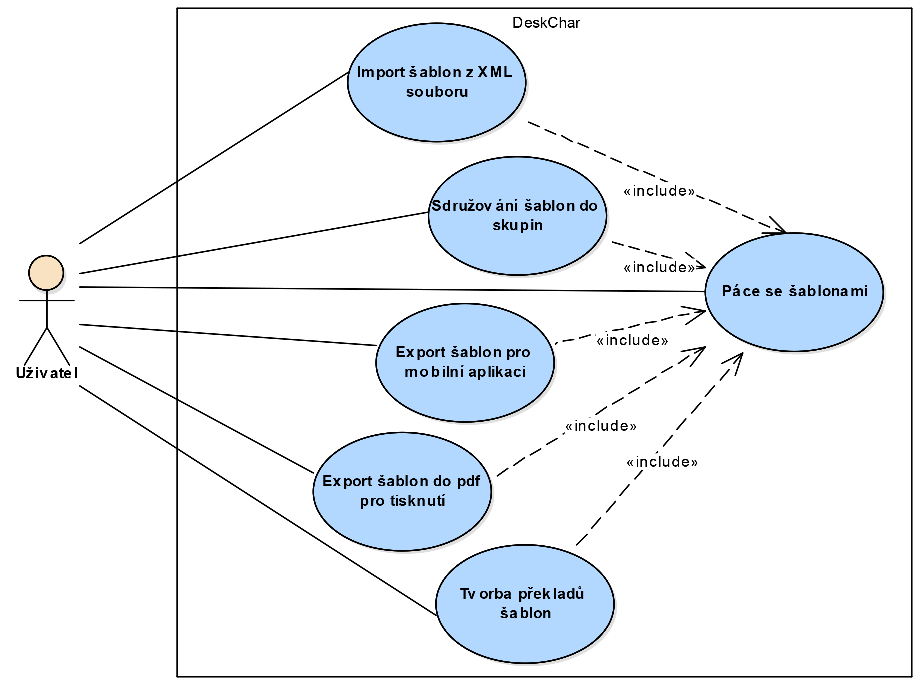
\includegraphics[width=0.8\textwidth]{images/usecase_sablony}
	\caption[Usecase šablony]{Ukázkový obrázek v~plovoucím prostředí}\label{fig:uc_sablony}
\end{figure}

Případ užití týkající se práci se šablonami namodelovaný na obrázku \ref{fig:uc_sablony} je oddělený od ostatních, protože obsahuje veškeré činnosti, které od aplikace vyžaduje hráč. Jedná se o~veškerou práci se šablonami pro mobilní aplikaci MobChar.\\
\\
\textbf{Vytváření a editace šablon:} uživatel si bude moci vytvořit nové šablony nebo editovat stávající. Veškeré parametry, které je možné do xml šablony zapsat, lze jednoduše upravovat v přehledném formuláři.\\
\\
\textbf{Import šablon z XML souboru:} program bude umožňovat import šablon ze strukturovaných xml souborů, které vytváří mobilní aplikace MobChar a samotný program. Importované šablony se přidají do databáze a lze je následně upravovat nebo překládat. \\
\\
\textbf{Sdružování šablon do skupin:} veškeré šablony půjde rozřazovat do stromové struktury pro větší přehlednost, pomocí vytváření složek a jednoduchého drag and drop systému. Takto rozřazené šablony budou umožňovat přehlednější práci a jednoduší export do xml souborů.\\
\\
\textbf{Export šablon:} veškeré vytvořené šablony lze z aplikace exportovat. K dispozici jsou různé druhy exportu. První možnost je export pro mobilní aplikace MobChar. Aplikace vytvoří strukturované XML soubory, které odpovídají formátu, který používá mobilní aplikace MobChar. Další možností exportu je PDF formát, který slouží pro tisknutí šablon do přehledného almanachu, který umožní využít šablony i hráčům, kteří mobilní aplikaci nemají nebo ji nechtějí použít. \\
\\
\textbf{Tvorba překladů šablon:} každá šablona může být přeložena do libovolného počtu jazyků. Při exportu šablon se všechny jazykové překlady exportují. Pomocí záložek se lze přepínat mezi jazyky.\\
\\
\subsection{Tvorba dobrodružství}
\begin{figure}\centering
	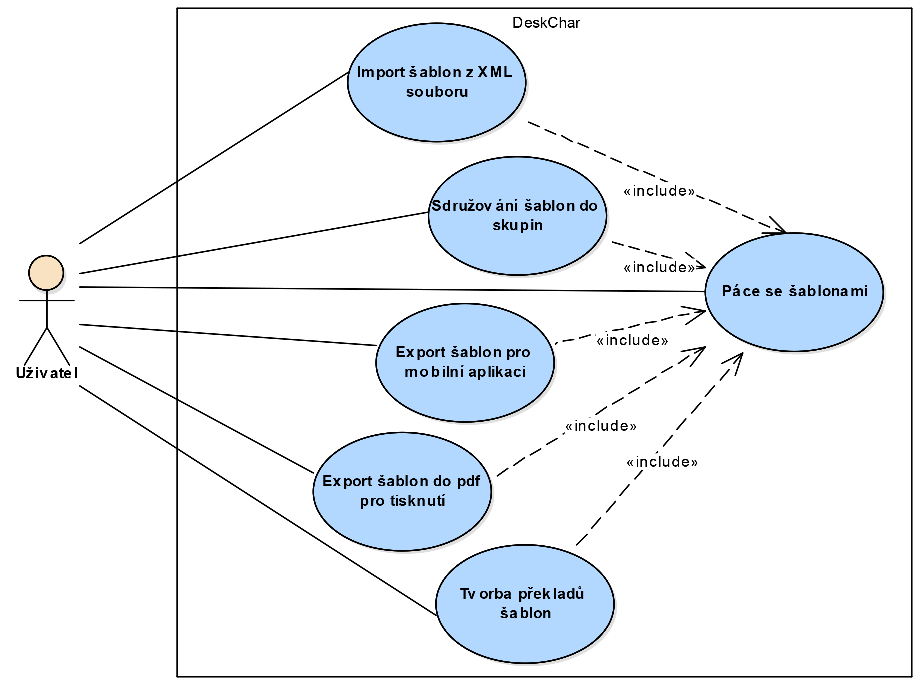
\includegraphics[width=0.8\textwidth]{images/usecase_sablony}
	\caption[Usecase šablony]{Ukázkový obrázek v~plovoucím prostředí}\label{fig:uc_sablony}
\end{figure}



\chapter{Návrh}

\chapter{Realizace}

\begin{conclusion}
	%sem napište závěr Vaší práce
\end{conclusion}

\bibliographystyle{csn690}
\bibliography{resources/mybibliographyfile}

\appendix

\chapter{Seznam použitých zkratek}
% \printglossaries
\begin{description}
	\item[HnH] Hra na hrdiny
	\item[DrD] Dračí doupě
	\item[RPG] Role-playing game
	\item[PJ] Pán jeskyně
	\item[DAO] Data access object
	\item[MobChar] Mobile character
	\item[DeskChar] Desktop character	
\end{description}

 

\chapter{Obsah přiloženého CD/USB}

%upravte podle skutecnosti

\begin{figure}
	\dirtree{%
		.1 readme.txt\DTcomment{stručný popis obsahu CD}.
		.1 exe\DTcomment{adresář se spustitelnou formou implementace}.
		.1 src.
		.2 impl\DTcomment{zdrojové kódy implementace}.
		.2 thesis\DTcomment{zdrojová forma práce ve formátu \LaTeX{}}.
		.1 text\DTcomment{text práce}.
		.2 thesis.pdf\DTcomment{text práce ve formátu PDF}.
		.2 thesis.ps\DTcomment{text práce ve formátu PS}.
	}
\end{figure}

\end{document}
